\documentclass[11pt]{article}
\usepackage[T1]{fontenc}
\usepackage[utf8]{inputenc}
\usepackage[margin=1in]{geometry}
\usepackage{amsmath,amssymb,amsthm,mathtools,booktabs,array}
\usepackage{microtype}
\usepackage{tikz}
\usetikzlibrary{positioning}
\usepackage[numbers,sort&compress]{natbib}
\usepackage[colorlinks=true,allcolors=blue]{hyperref}
\newcommand{\R}{\mathbb{R}}
\newcommand{\Q}{\mathbb{Q}}
\newcommand{\ER}{\exists\mathbb{R}}
\newcommand{\NP}{\mathsf{NP}}
\newcommand{\PSPACE}{\mathsf{PSPACE}}
\newcommand{\RPF}{\textnormal{\textsc{RPF}}}
\newcommand{\ACPF}{\textnormal{\textsc{ACPF}}}
\newcommand{\ETRINV}{\textnormal{\textsc{ETR-INV}}}
\newcommand{\power}{\mathcal{P}}
\newcommand{\comp}[1]{\overline{#1}}
\newtheorem{theorem}{Theorem}[section]
\newtheorem{lemma}[theorem]{Lemma}
\newtheorem{proposition}[theorem]{Proposition}
\newtheorem{corollary}[theorem]{Corollary}
\theoremstyle{definition}
\newtheorem{definition}[theorem]{Definition}
\theoremstyle{remark}
\newtheorem{remark}[theorem]{Remark}

\title{Exact Feasibility of Resistive Power Networks}
\author{}
\date{}
\begin{document}
\maketitle
\begin{abstract}
We prove that feasibility of a resistive power network with positive voltage
intervals and signed power-injection intervals is complete for the existential
theory of the reals. The result holds on simple graphs of maximum degree three,
with conductances in $\{1,2\}$ and all interval endpoints from fixed finite sets.
The reduction implements bounded addition and inversion using voltage-pinned
buses and complement paths. It preserves the solution set by a rational
bijection whose inverse reads designated bus voltages. Consequently, polynomial-size
certificates for exact feasibility verifiable in deterministic polynomial time
would imply $\NP=\ER$.
\end{abstract}
\section{Exact feasibility and the resistive model}
\label{sec:foundations}

In a resistive network, current depends linearly on bus voltages, but power is
the product of voltage and current. This distinction makes exact feasibility a
quadratic problem even when the network has no discrete controls. We study its
complexity with interval restrictions on both voltage and net power injection.
The model concerns direct-current electrical networks; it is distinct from
the linear ``DC approximation'' of an alternating-current network.

\subsection{Input model and complexity convention}

Let $G=(N,E)$ be a finite simple undirected graph. Each line $\{i,j\}\in E$
has conductance $g_{ij}=g_{ji}\in\Q_{>0}$. Bus $i$ has voltage bounds
$0<\ell_i\le u_i$ and injection bounds $p_i^-\le p_i^+$, all rational and
finite. Its net injection at voltage vector $v\in\R^N$ is
\begin{equation}
 \power_i(v)=v_i\sum_{j:\{i,j\}\in E}g_{ij}(v_i-v_j).
 \label{eq:rpf}
\end{equation}
An injection is positive for net supply to the network and negative for net
withdrawal. An isolated bus has injection zero. The decision problem $\RPF$
asks whether
\begin{equation}
 \ell_i\le v_i\le u_i,\qquad
 p_i^-\le\power_i(v)\le p_i^+\qquad(i\in N)
 \label{eq:rpf-bounds}
\end{equation}
has a solution. Singleton intervals are allowed. We impose neither additional
line-flow limits nor a requirement that an injection be fixed whenever a
voltage is variable. Thus the input permits voltage-pinned buses with fixed
injections, variable-voltage buses with fixed injections, and buses with both
quantities in intervals. These choices are material to the reduction.

The graph and its rational data are encoded in binary. The existential
theory of the reals, denoted ETR, asks whether an existentially quantified
Boolean combination of polynomial equalities and inequalities with integer
coefficients is true. The class $\ER$ consists of decision problems reducible
to ETR by polynomial-time many-one reductions. Rational coefficients are
equivalent: each atomic constraint can have its denominators cleared using
a positive integer of polynomial bit length. We use the Turing model of
computation and the standard inclusions
\begin{equation}
 \NP\subseteq\ER\subseteq\PSPACE.
 \label{eq:complexity-inclusions}
\end{equation}
See \citet[Section 1.1]{AbrahamsenMiltzow2019} for these conventions and their
background. Exact feasibility quantifies over real solutions, not over decimal
approximations. An irrational solution alone does not rule out membership in
$\NP$: a certificate need not list rational bus voltages.

\begin{proposition}
\label{prop:rpf-membership}
The problem $\RPF$ belongs to $\ER$.
\end{proposition}
\begin{proof}
Equations~\eqref{eq:rpf}--\eqref{eq:rpf-bounds} form a conjunction of rational
polynomial inequalities of degree at most two in $|N|$ real variables.
Writing each incident-line term explicitly uses $O(|N|+|E|)$ terms and
polynomially many bits. Clearing denominators gives an ETR instance.
\end{proof}

The model respects the usual dissipation identity:
\begin{equation}
 \sum_{i\in N}\power_i(v)
 =\sum_{\{i,j\}\in E}g_{ij}(v_i-v_j)^2\ge0.
 \label{eq:dissipation}
\end{equation}
Indeed, the two terms of a line sum to $g_{ij}(v_i-v_j)^2$.
The injection intervals, rather than a separate balance equation with zero
total injection, account for these losses. In particular, permitting signed
injections does not remove physical power balance.

\subsection{The bounded arithmetic source problem}

An instance of $\ETRINV$ consists of named variables $x_1,\ldots,x_n$,
each restricted to $[1/2,2]$, and a conjunction of equations of the forms
\begin{equation}
 x=1,\qquad x+y=z,\qquad xy=1.
 \label{eq:etr-inv}
\end{equation}
Variable names in an equation may coincide. The interval restrictions are
part of feasibility, not a promise that all real solutions already lie there.
Abrahamsen, Adamaszek, and Miltzow prove this problem $\ER$-complete
\citep[Definition 5 and Theorem 7 of the STOC/arXiv version]{AbrahamsenEtAl2018}.
The journal version is \citet{AbrahamsenEtAl2022}.
Replacing each equation $x=1$ by $x x=1$ preserves the solution set, since
$x>0$. Hence we use only addition and inversion equations below.
Let $S_\Phi\subseteq[1/2,2]^n$ denote the solution set of the normalized
instance $\Phi$, and let $m$ be its number of equations.
We retain all named variables, including those occurring in no equation.

\section{A bounded-degree reduction with fixed numerical data}
\label{sec:resistive}

\begin{theorem}
\label{thm:rpf-complete}
The problem $\RPF$ is $\ER$-complete. Hardness holds for simple graphs with
maximum degree three, conductances in $\{1,2\}$, voltage intervals in
\[
 \bigl\{[1/2,2],\ [1,1],\ [1,4]\bigr\},
\]
and injection intervals in
\[
 \bigl\{[-85,85],\ [-1/2,-1/2],\ [1/2,1/2],\
 [-5/2,-5/2],\ [-1,-1]\bigr\}.
\]
For an instance of $\ETRINV$ with $n$ named variables and $m$ equations,
the reduction constructs at most $n+16m$ buses and $18m$ lines.
\end{theorem}

The construction uses a voltage-pinned bus to impose a linear relation on
its neighbors, and one variable-voltage bus to impose inversion.
Copying values along paths keeps the degree bounded even when a variable
occurs arbitrarily often. Throughout this section, a \emph{free injection}
means the fixed interval $[-85,85]$, not an unbounded or omitted constraint.

\subsection{Pinned buses and the supply of distinct value copies}
\label{subsec:copies}

A \emph{value bus} has voltage interval $[1/2,2]$ and free injection.
A \emph{pinned bus} has voltage $1$ and a specified injection $p$.
If its distinct neighbors carry voltages $a_1,\ldots,a_d$ with conductances
$h_1,\ldots,h_d$, its equation is
\begin{equation}
 \sum_{r=1}^d h_r(1-a_r)=p.
 \label{eq:pinned}
\end{equation}
In particular, a pinned bus $C$ with injection $-1/2$ and two unit-conductance
lines enforces $a+b=5/2$. Write $\comp{x}=5/2-x$; the map $x\mapsto\comp{x}$
is an involution of $[1/2,2]$.

For each variable $x$ begin with a value bus $X_x$. Successively extending a
path
\begin{equation}
 X_x\mathbin{\text{---}} C_1\mathbin{\text{---}}\comp{X}_x\mathbin{\text{---}}C_2\mathbin{\text{---}}X'_x\mathbin{\text{---}}\cdots
 \label{eq:copy-chain}
\end{equation}
supplies alternating voltages $x,\comp{x},x,\ldots$.
Each $C_r$ has voltage $1$, injection $-1/2$, and exactly its two path lines.
Every value bus may receive at most one further line from an equation gadget.
Here is a deterministic allocation rule. Maintain the current end of each
path, its parity (plain or complemented), and whether its one gadget slot is
unused. On a request for a copy, extend the path until the end has the requested
parity and an unused slot; allocate that slot and continue from this end for
the next request. Each extension adds one pinned bus, one value bus, and two
lines. At most two extensions are needed per request. All requested copies
are distinct, even if they represent the same variable in the same equation.
Unused named variables retain their single isolated bus $X_x$.

\subsection{Addition and inversion gadgets}

For $x+y=z$, introduce a pinned bus $A$ with injection $1/2$ and three
unit-conductance lines to fresh requested copies of $x$, $y$, and
$\comp{z}$. Its equation is
\[
 (1-x)+(1-y)+(1-\comp{z})=1/2
 \quad\Longleftrightarrow\quad x+y=z.
\]
For $x+x=z$ the two plain copies of $x$ are distinct buses. The same allocation
rule covers $x+y=x$ and $x+x=x$; such equations are correctly infeasible in
the positive source interval.

For $xy=1$, introduce buses $I,W,C_I,D$ with the data in
Table~\ref{tab:inversion}. Request three distinct complemented value buses:
two for $x$ and one for $y$. Connect them as in Figure~\ref{fig:inversion}.
If $x=y$, all three still have distinct bus identities.

\begin{table}[htbp]
\centering
\begin{tabular}{@{}clll@{}}
\toprule
Bus & Voltage interval & Injection interval & Neighbors (conductance)\\
\midrule
$I$ & $[1/2,2]$ & $[-1,-1]$ & $W$ (1), $C_I$ (1)\\
$W$ & $[1,4]$ & $[-85,85]$ & $I$ (1), $D$ (1)\\
$C_I$ & $[1,1]$ & $[-1/2,-1/2]$ & $I$ (1), first $\comp{x}$ copy (1)\\
$D$ & $[1,1]$ & $[-5/2,-5/2]$ & $W$ (1), second $\comp{x}$ copy (2), $\comp{y}$ copy (1)\\
\bottomrule
\end{tabular}
\caption{The four new buses for an inversion equation $xy=1$.}
\label{tab:inversion}
\end{table}

\begin{figure}[htbp]
\centering
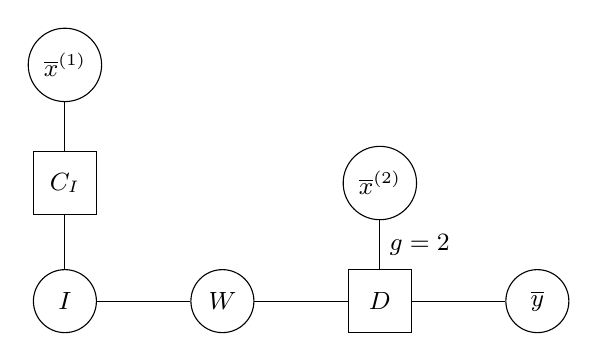
\begin{tikzpicture}[every node/.style={font=\small},
 bus/.style={circle,draw,minimum size=8mm},
 pin/.style={rectangle,draw,minimum size=8mm}]
\node[bus] (I) at (0,0) {$I$};
\node[bus] (W) at (2,0) {$W$};
\node[pin] (D) at (4,0) {$D$};
\node[pin] (C) at (0,1.5) {$C_I$};
\node[bus] (x1) at (0,3) {$\comp{x}^{(1)}$};
\node[bus] (x2) at (4,1.5) {$\comp{x}^{(2)}$};
\node[bus] (y) at (6,0) {$\comp{y}$};
\draw (x1)--(C)--(I)--(W)--(D)--(y);
\draw (D)--node[right] {$g=2$}(x2);
\end{tikzpicture}
\caption{Inversion gadget. Squares have voltage $1$; the three upper or
rightmost value copies belong to variable paths, whose lines are omitted.
Every unmarked line has conductance $1$. Superscripts distinguish buses,
not numerical values.}
\label{fig:inversion}
\end{figure}

The equation at $C_I$ gives
\[
 (1-v_I)+(1-\comp{x})=-1/2,
 \qquad\text{hence }v_I=x.
\]
The injection equation at $I$ is therefore
\begin{equation}
 x\bigl[(x-v_W)+(x-1)\bigr]=-1,
 \qquad v_W=2x-1+1/x.
 \label{eq:inversion-I}
\end{equation}
Division is valid because $x\ge1/2$. At $D$ the equation reads
\begin{equation}
 (1-v_W)+2(1-\comp{x})+(1-\comp{y})=-5/2
 \quad\Longleftrightarrow\quad y=v_W-2x+1.
 \label{eq:inversion-D}
\end{equation}
Together these equations imply $y=1/x$.

Conversely, if $x,y\in[1/2,2]$ and $xy=1$, set $v_I=x$ and
$v_W=h(x):=2x-1+1/x$. Both pinned-bus equations and the injection equation
at $I$ then hold. The voltage bound on $W$ is valid: on $[1/2,2]$,
$h'(x)=2-x^{-2}$ and $h''(x)=2x^{-3}>0$, so its minimum is
$2\sqrt{2}-1$ at $1/\sqrt{2}$ and its maximum is the larger endpoint value,
$h(2)=7/2$. Thus
\begin{equation}
 1<2\sqrt{2}-1\le v_W\le7/2<4.
 \label{eq:W-range}
\end{equation}

\subsection{The complete network and proof of equivalence}

Construct all variable paths and equation gadgets with the allocation rule
above. Path value buses have at most two path lines and one gadget line.
Path pinned buses and $C_I$ have degree two; addition buses and $D$ have
degree three; $I$ and $W$ have degree two. Distinct requested copies and fresh
gadget buses prevent loops and parallel edges. Consequently $G$ is simple and
its maximum degree is three.

Every bus voltage belongs to $[1/2,4]$ and every conductance is at most $2$.
For every voltage vector in the prescribed box, not just the intended
solutions, a free-injection bus satisfies
\begin{equation}
 |\power_i(v)|
 \le v_i\sum_{j:\{i,j\}\in E}g_{ij}|v_i-v_j|
 \le 4\cdot3\cdot2\cdot\frac72=84<85.
 \label{eq:free-bound}
\end{equation}
The free-injection intervals therefore add no restriction inside that box.

\begin{lemma}
\label{lem:reduction-equivalence}
The constructed network is feasible if and only if $S_\Phi\ne\varnothing$.
More precisely, restriction to $(v_{X_x})_{x= x_1,\ldots,x_n}$ is a bijection
from its feasible voltage set onto $S_\Phi$.
\end{lemma}
\begin{proof}
Given a feasible voltage vector, put $x=v_{X_x}$ for each named variable.
Every path pinned bus has exactly its two prescribed neighbors, so its
equation forces successive values to be complementary. Every requested copy
thus has its specified value. The addition equation yields $x+y=z$; equations
\eqref{eq:inversion-I}--\eqref{eq:inversion-D} yield $xy=1$. This recovers a
point of $S_\Phi$.

Conversely, given a point of $S_\Phi$, assign alternating values $x$ and
$5/2-x$ along each variable path, voltage $1$ to every pinned bus, and
$v_I=x$, $v_W=2x-1+1/x$ in each inversion gadget. The preceding algebra
verifies every fixed-injection equation. The voltage bounds follow from the
source interval and~\eqref{eq:W-range}; the remaining injection bounds follow
from~\eqref{eq:free-bound}. An isolated $X_x$ has injection zero and retains
exactly the unconstrained source coordinate $x\in[1/2,2]$.

Finally all bus voltages have been uniquely determined by the recovered
source coordinates: path values alternate, pinned values are fixed, and
\eqref{eq:inversion-I} determines $W$. These two maps are inverse bijections.
\end{proof}

\begin{proof}[Proof of Theorem~\ref{thm:rpf-complete}]
Each equation requests exactly three value copies. With at most two path
extensions per request, the paths contribute at most $12m$ new buses and
$12m$ lines in addition to the $n$ initial buses. An addition adds one
further bus and three lines; an inversion adds four further buses and six
lines. Hence the stated bounds $n+16m$ and $18m$ hold, including unused
variables. All numerical data are exactly those displayed in the theorem.
The number of objects is linear in $n+m$; encoding their indices uses
$O((n+m)\log(n+m+2))$ bits, and the construction is polynomial-time.
Lemma~\ref{lem:reduction-equivalence} and $\ER$-completeness of $\ETRINV$
give hardness. Proposition~\ref{prop:rpf-membership} gives membership.
\end{proof}

\begin{proposition}[Preservation of the solution set]
\label{prop:rational-bijection}
The extension map from source solutions to feasible network voltages in
Lemma~\ref{lem:reduction-equivalence} is a homeomorphism whose forward and
inverse coordinate functions are rational with rational coefficients.
Its inverse is restriction to the buses $X_x$, a coordinate projection.
\end{proposition}
\begin{proof}
The extension map has coordinate functions $x$, $5/2-x$, $1$, and
$2x-1+1/x$. They are rational and continuous because $x\ge1/2$.
The inverse projection is linear and continuous. The statement also holds
for empty solution sets and for unused source coordinates.
\end{proof}

\begin{corollary}
\label{cor:rpf-np}
If $\RPF$ belongs to $\NP$, then $\NP=\ER$. In particular, unless these
classes coincide, not every feasible rational instance has a polynomial-size
certificate verifiable in deterministic polynomial time. The problem belongs
to $\PSPACE$.
\end{corollary}
\begin{proof}
By completeness every problem in $\ER$ reduces to $\RPF$. Membership of
$\RPF$ in $\NP$ would imply $\ER\subseteq\NP$, and
\eqref{eq:complexity-inclusions} gives equality. The certificate formulation
is the definition of $\NP$; the space upper bound follows from the same
inclusions.
\end{proof}

The fixed-data conclusion is stronger than a claim that large numerical
coefficients can be encoded economically: all numerical choices in the
hard instances come from finite sets independent of instance size. Their
combinatorial incidence pattern carries the growing input. The theorem uses
general graphs and signed injection intervals; it makes no assertion here
about a load-only model or a tree restriction.

\bibliographystyle{plainnat}
\bibliography{references}
\end{document}
